\section{Single Robot Method Comparison}
\label{sec:04_tdoaSingle}

For comparability of the results, one exemplary measurement is utilized
to present and analyse the \ac{TDOA} methods.
In this data set, the sound source is placed at the right front
of the robot with 4.5\si{m} distance.
This corresponds to an an angle of -33.7\si{\degree} in robot coordinates.
Some samples around the signal start of the received signal data
is plotted in \ref{fig:04_tdoaSignal} for all channels.
% -------------------------------------------------------------
\begin{figure}[ht]
	\centering
		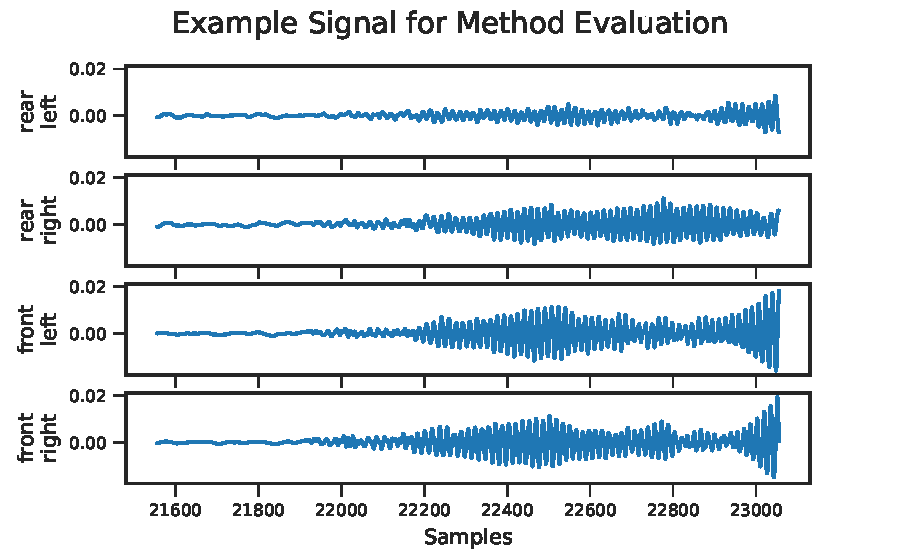
\includegraphics[]{figures/evaluation/cc_frontRight_1_signal}
	\caption{Signal start section of a whistle sound recorded from front right.}
	\label{fig:04_tdoaSignal}
\end{figure}
% -------------------------------------------------------------

As the next sections focus on the performance of the \ac{TDOA} methods,
the start index is set manually.
A frame size is defined with 256 samples and is selected around the start index for
the correlation methods as explained in \cref{sec:03_tdoa}.
For the phase method, the first frame with a size of 64 samples
is chosen where a whistle is detected in all channels.

In the following, the correlation function $R_{x_ax_b}$ of two signals
$x_a$ and $x_b$ as in \cref{chap:02_prerequisites} is shortened
to $R_{ab}$ for simplicity.


\subsection{Cross Correlation}
\label{subsec:04_ccSingle}
% -------------------------------------------------------------

To visualize the result of the \ac{CC}, the correlations are plotted in
\cref{fig:04_cc}. For $R_{23}$ and $R_{13}$ the peak is clearly traceable.
However, for the other \ac{CC} the problem of a low maximum peak
arises as mentioned in \cref{sec:02_cc}.
% -------------------------------------------------------------
\begin{figure}[ht]
	\centering
		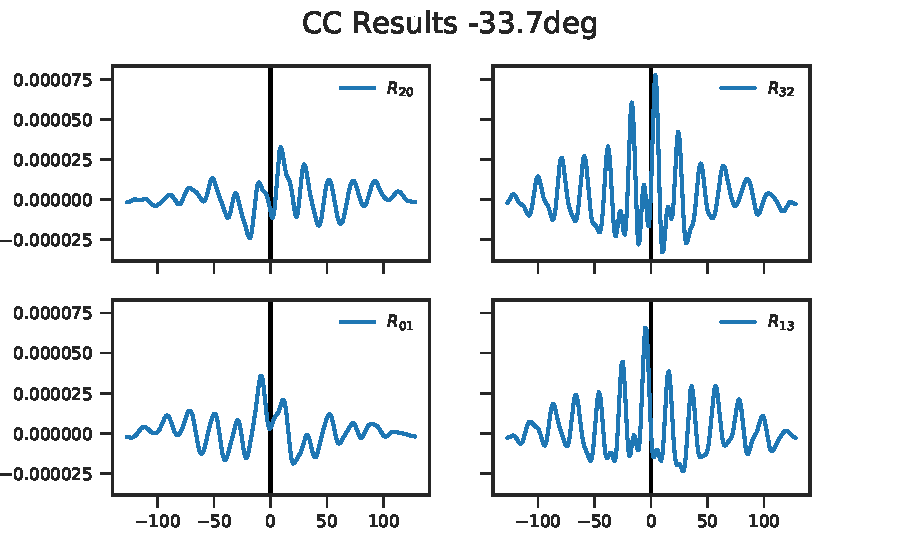
\includegraphics[]{figures/evaluation/cc_frontRight_1}
	\caption{Cross correlation results of signal from front right (-33,7\si{\degree}).}
	\label{fig:04_cc}
\end{figure}
% -------------------------------------------------------------
\btline{ht}{1.2}
\btab{|c|c|c|c|c|}
\hline
Base Channel & Next Channel & Delay & Candidate (-) & Candidate (+)\\
\hline
0 & 1 & -8.25 & -144.9 & -35.1\\
\hline
1 & 3 & -4.59 & -17.4 & 78.6\\
\hline
2 & 0 & 9.16 & -30.6 & -30.6\\
\hline
3 & 2 & 3.94 & -150.2 & -29.8\\
\hline
\etab
\et{Cross correlation delay results of singal from front right}{04_cc}
% -------------------------------------------------------------

According to the delays in \cref{tab:04_cc}, the final result of the \ac{CC}
is -26.9\si{\degree} which emerges an error of 6.8\si{\degree}.
The delay between channel 2 and 0 is larger than the maximal delay of 6.85 samples
and therefore cut to the maximal sample delay.
Besides these, the \ac{TDOA} between the channel pairs produce one appropriate
direction candidate which correctly points to the sound source.
% -------------------------------------------------------------

\subsection{Generalized Cross Correlation}
\label{subsec:04_gccSingle}
% -------------------------------------------------------------
\Cref{fig:04_gcc} presents the cross correlation result by the \ac{GCC} method of
the same signal data as in the previous section.
The subsample delays for each channel pair and their resulting direction candidates
are listed in \cref{tab:04_gcc}.
From this, a final direction of -30.0\si{\degree} is determined
resulting in an error of 3,69\si{\degree}.
It is apparent that the peaks of the \ac{GCC} are better to detect than the peaks of the
\ac{CC}.
% -------------------------------------------------------------
\begin{figure}[ht]
	\centering
		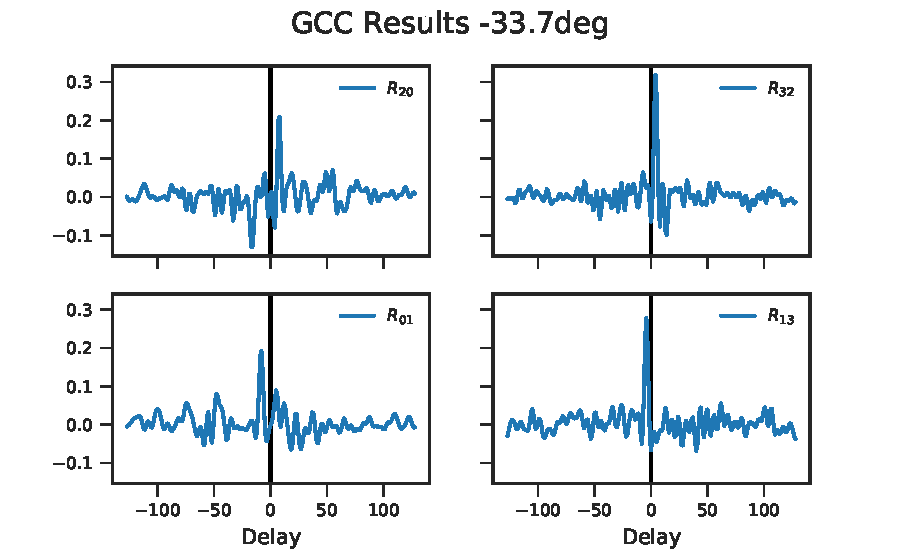
\includegraphics[]{figures/evaluation/gcc_frontRight}
	\caption{Generalized cross correlation results of signal from front right.}
	\label{fig:04_gcc}
\end{figure}
% -------------------------------------------------------------
\btline{ht}{1.2}
\btab{|c|c|c|c|c|}
\hline
Base Channel & Next Channel & Delay & Candidate (-) & Candidate (+)\\
\hline
0 & 1 & -8,28 & -144,7 & -35,3\\
\hline
1 & 3 & -4,09 & -22,8 & 84,0\\
\hline
2 & 0 & 7,60 & -30.6 & -30.6\\
\hline
3 & 2 & 4,13 & -148,7 & -31,3\\
\hline
\etab
\et{Generalized cross correlation delay results of singal from front right}{04_gcc}
% -------------------------------------------------------------
\subsection{Phase Difference}
\label{subsec:04_phaseSingle}

For detecting the source direction with phase difference, a smaller frame
size of 64 samples is set.
Previously, two cases were introduced in \cref{subsec:03_phase} where either a
fixed frequency is focused on or the frequency with maximal magnitude is
taken for reference.

First, the result of the dynamically selected frequency is presented.
As stated in the implementation chapter, the frame is chosen where the
frequencies of the maximal amplitudes coincides for all channel which is
at 2756,25\si{\hertz}.
In the upper plot of \cref{fig:04_phaseSingle} one sees the received samples which
will be transformed into frequency domain by \ac{FFT} and using a Hann window.
The resulting phases and amplitudes are listed in \cref{tab:04_phaseSingle}.
For comprehensibility, the determined frequency information visualized by
wave signals with these phases and amplitudes
in the lower subplot of \cref{fig:04_phaseSingle}.
Due to the larger distance between channels 0 and 1, the phase difference
information is neglected.
Outcome from the applied phase differences is -29,2\si{\degree} by the combination of
-17,6\si{\degree}, -30,6\si{\degree} and -39,3\si{\degree}.
% -------------------------------------------------------------
\btline{ht}{1.2}
\btab{|c|c|c|}
\hline
Channel & Phase [\si{\deg}] & Amplitude\\
\hline
0 & -1,55 & 0,00144\\
\hline
1 & -177,7 & 0,00287\\
\hline
2 & 173,4 & 0,00279\\
\hline
3 & -75,0 & 0,00372\\
\hline
\etab
\et{Phase and amplitude of frame signals with 2756,25Hz}{04_phaseSingle}
% -------------------------------------------------------------
\btline{ht}{1.2}
\btab{|c|c|c|c|c|}
\hline
Base Channel & Next Channel & Phase Difference & Candidate (-) & Candidate (+)\\
& & [\si{\deg}] & [\si{\deg}] & [\si{\deg}] \\
\hline
0 & 1 & 176,2 & 33,07 & 146,9\\
\hline
1 & 3 & -102,7 & -17,6 & 78,8\\
\hline
2 & 0 & 173,4 & -30,6 & -30,6\\
\hline
3 & 2 & 113,1 & -140,7 & -39,3\\
\hline
\etab
\et{Phase differences and resulting direction candidates of example data with phase method}{04_phaseDiffSingle}
% -------------------------------------------------------------
\begin{figure}[ht]
	\centering
		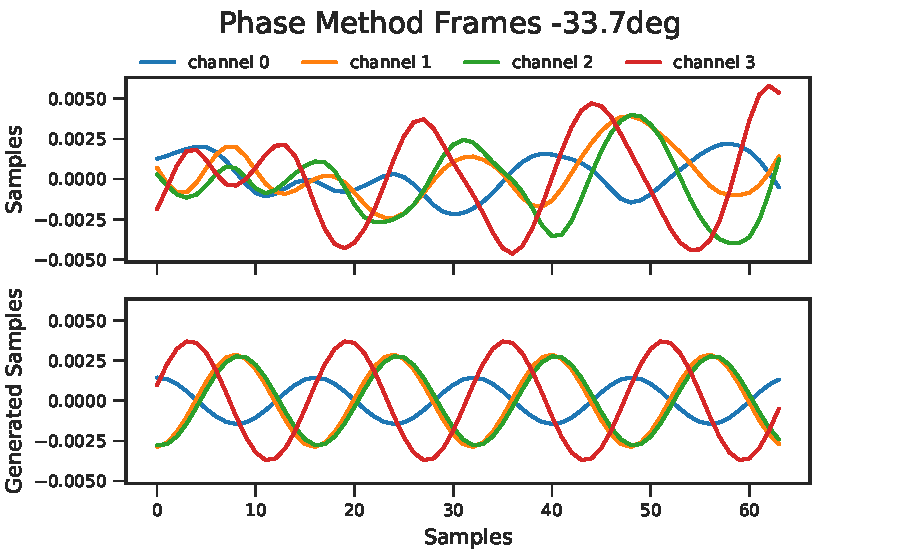
\includegraphics[]{figures/evaluation/phase_cos}
	\caption{Frames used for the direction detection by phase method.}
	\label{fig:04_phaseSingle}
\end{figure}
% -------------------------------------------------------------

Secondly, the frequency to examine $f_c$ is set to the first represented frequency
larger than 2600\si{\hertz} which is 2627,1\si{\hertz} at a \ac{FFT} length
of 256.
At this frequency, outcome of the direction candidates listed in \cref{tab:04_fixedFreqResult}
with the considered delays is -29,6\si{\degree}.
% -------------------------------------------------------------
\btline{ht}{1.2}
\btab{|c|c|c|c|c|}
\hline
Base Channel & Next Channel & Phase Difference & Candidate (-) & Candidate (+)\\
& & [\si{\deg}] & [\si{\deg}] & [\si{\deg}] \\
\hline
1 & 3 & -79,1 & -26,8 & 88,0\\
\hline
2 & 0 & 167,7 & -30,6 & -30,6\\
\hline
3 & 2 & 88,5 & -148,7 & -31,3\\
\hline
\etab
\et{Resulting candidates of phase difference method with fixed frequency
	2411,72Hz of example measurement from front right
	(-33,3\si{\degree})}{04_fixedFreqResult}
% -------------------------------------------------------------
% Configuration for Phase Method
\subsection{Fixed Frequency Value}
\label{subsec:04_fixedFrequencyVal}

In order to decide on a fixed frequency for the phase method,
resulting errors of different frequency were evaluated.
For this, all measurements in \cref{subsec:04_labMeasurements}
of the robot 26 at the center point are utilized.
As the \ac{RMSE} in \cref{fig:04_diffFc} shows, for frequencies smaller
than 2600\si{\hertz} the errors are much higher.
With a frequency of 2024.12\si{\hertz}, error is largest.
The fixed frequency is set to 2627,1\si{\hertz} according
to the smallest \ac{RMSE}.
% -------------------------------------------------------------
\begin{figure}[ht]
	\centering
		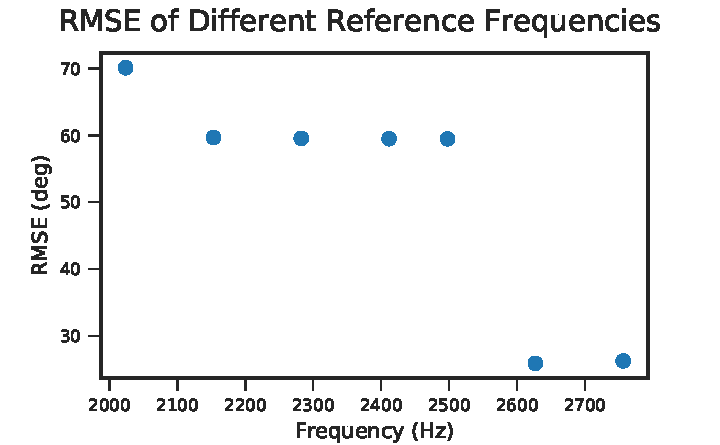
\includegraphics[]{figures/evaluation/phase_fc_rmse}
	\caption{Result of all measurements for Nao 26 to compare different
	fixed frequency values.}
	\label{fig:04_diffFc}
\end{figure}
% -------------------------------------------------------------
\subsection{Frame Number}
\label{subsec:04_frameNumber}

Not only does the frequency play a role for the phase method,
but also the frame chosen.
To evaluate if the result changes over time, the frame to
utilize is shifted by half the frame size for all measurements
of \cref{subsec:04_labMeasurements} for the robot at the center
point.
% [ 29.08029745  58.1426789   65.27548831  67.91984464  76.82890558
%   97.33976251  96.63736674 100.2203543  105.14752253  61.28179302
%   60.0017076   50.60063622  53.80158271  49.0830362   62.64453085]
In \cref{fig:04_phaseOverTime} we see, that the first channel frames
with zero shift gives the best result with a \ac{RMSE} of 29,1\si{\degree}.
This again shows us, that the signal start detection plays a
large role for the correct result.
% -------------------------------------------------------------
\begin{figure}[ht]
	\centering
		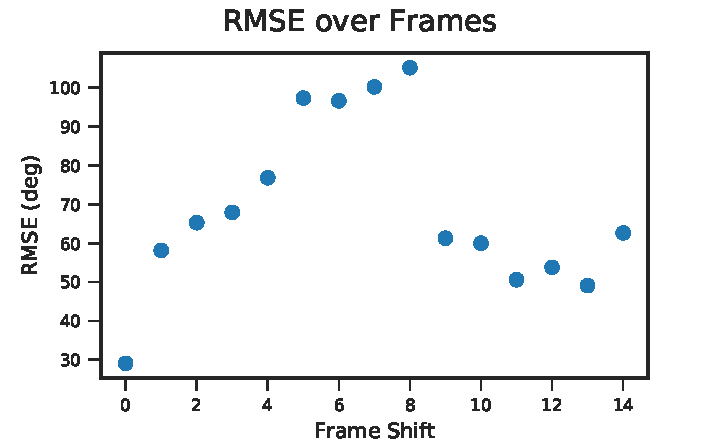
\includegraphics[]{figures/evaluation/phase_over_time}
	\caption{}
	\label{fig:04_phaseOverTime}
\end{figure}
% -------------------------------------------------------------